\documentclass[12pt]{article}

%Packages
\usepackage{graphicx}
\graphicspath{ {/} }
\usepackage{amsmath}
\usepackage{wrapfig}
\usepackage[utf8]{inputenc}
\usepackage{lmodern}
\usepackage{setspace}
\usepackage{float}
\usepackage{sidecap}
\doublespacing
\usepackage{geometry}
\geometry{letterpaper,margin=1in}
\title{Engineering 031 Capstone}
\author{Ethan Blackwood, Lotanna Ezenwa}
\date{\today{}}

\begin{document}

\pagenumbering{arabic}
\maketitle
\begin{abstract}
This study shows the implementation of a microphone-speaker system using digital signal processing methods on a Nexys 3 Spartan-6 FPGA Board. The hardware used, in addition to the Nexys 3 FPGA, were a PMOD Mic+A/D Converter, a PMOD D/A Converter, a PMOD Amplifier 1/8", and a standard 1/8" speaker. We implemented simultaneous filtering, looping, and reverberation effects only using the RAM on the Spartan-6 XC6LX16-CS324. Our approach was to create the system in a modular and efficient manner that remains scalable and customizable. At completion of the project, we found that our microphone-speaker system can produce looping and mixing effects at CD-R qualities without using additional on-board memories.

\end{abstract}
\newpage
\tableofcontents
\newpage
\section{Introduction}
\paragraph{}
Digital signal processing (DSP) methods are a fundamental component of modern communication, data transfer, and acoustics. The basis of this is converting signals between analog and digital representations. Once an analog signal has been converted to its digital representation, mathematical operations can be applied to transform the signal. These tranformations may produce various effects that are heard when the signal is converted to to an analog signal through a speaker.
\paragraph{}
Sampling is the process of constructing a digital signal through approximations of discrete sections of an analog signal. Logically, a high number of samples leads to a better approximation of the analog signal. A high sampling rate, measured in Hz, produces a higher quality of sound out of the speaker, but requires more storage to hold the samples per unit of time. A compact microphone-speaker system using only internal memory has to compromise sound quality, signal size, or processing effects when processing the microphone signals. We introduce a Spartan 6 FPGA Implementation that be configured to produce varying configurations of sound qualities, recording lengths, and sound effects.

\section{Design Solution}

\subsection{Specifications}
\paragraph{}
Our audio circuit creates a microphpone-speaker system with controllable and layerable effects. To do this, it uses on-board input switches and buttons to enable, control, and modify the modular effect circuits through which it passes audio samples. These samples are output at the speaker to produce the configured effects.
\paragraph{}
On the board, there are 3 control switches, 4 control buttons, and 4 status LEDs. There is also a PMOD Microphone, a D/A Converter, a 1/8" audio jack and amplifier, and a 1/8" Speaker. 
\begin{wrapfigure}{r}{0.5\textwidth}
\includegraphics[width=0.5\textwidth]{front_panel.eps}
\caption{Our Front Panel}
\end{wrapfigure}



\subsection{Operating Instructions}
\paragraph{}
To set up the microphone, plug the PMOD Microphone (with buffer) into the 6-pin cable extension. Attach a 6-pin male-male connector to the opposite end of the cable extention. Plug this end of the cable into the top 6 pins of the JA PMOD expansion port, keeping the pin orientation consistent with the pins on the PMOD microphone (VCC to VCC).



\paragraph{}
To set up the speaker, plug the PMOD D/A Converter into the top 6 pins of the JB PMOD expansion port. Take the PMOD Amplifier + 1/8" Audio port and bend pins 2 and 4 to allow a parallel connection with a separate cable extender. Plug a 6-pin male-male adapter to the opposite end of the cable extender. Plug this cable extension into the JC PMOD expansion port, keeping the pin orientation consistent. Plug the PMOD Amplifier + 1/8" Audio port into the D/A converter, keeping the pin orientation consistent. Finally, plug the speaker into the 1/8" audio jack on the PMOD Amplifier + 1/8" Audio port. 

\paragraph{}
To configure the microphone speaker system, change the REVERB STRENGTH, LOOPER WIDTH, BIT DEPTH, and BITRATE constant parameters in the top-level .vhd file prior to synthesis. These control the effects and quality of the audio signals translated through the circuit. Once the FPGA has been programmed, turn on the speaker via its on-board switch. This is the basic microphone function of the system. The reverberation and looper can be enabled via their own switches. 

\paragraph{}
With the looper enabled, LEDs will begin to sequentially turn on. The center button erases the current loop and begins recording sound to the start of RAM. When the looper is recording, the recording LED will illuminate. To increase or decrease speed of the loop, press the up and down buttons on the Nexys 3, respectively. To add a track, press the rightmost button on the Nexys 3. 

\subsection{Theory of Operation}
\paragraph{}
Our design conserves memory by continuosly routing the input from the microphone through our chosen effects, storing data only when an effect requires it. The entire system consists of the A/D Converter, the Looper, the Reverberator, and the D/A Converter. 

\paragraph{}
The A/D Converter processes the analog audio signal into its digital representation. Our circuit uses a start-sample bit to query the PMOD Microphone for a 12-bit sample at 12.5Mhz. The A/D Converter outputs an enable bit to the sampling chip on the PMOD Microphone. The Microphone sends 4 "0"s as start bits, then serially fills the rest of a 16-bit shift register with a 12-bit sample. The register is then truncated to 12-bits and sent to the looper along with a high bit to signal when the sample is completed. The A/D Converter also outputs a synchronization clock to signal the time at which each bit from the sample is shifted. 
\paragraph{}
The Looper takes this 12-bit sample as an input, and reroutes it depending on the input switches from the board. The outputs are looped audio signals and status LEDs, and status bits. Internally, the looper has a controller, RAM, and two up-counters whose size can be changed easily at synthesis. The controller  handles the I/O bit logic in the circuit. When the looper is disabled via its switch, the input audio sample is routed directly to the output.
\paragraph{}
When the looper is enabled, it reads sequentially from the RAM while still taking in audio samples. The looper adds the input signal to the signal from its RAM, the outputs the result. It also continuously calculates how far it has read through its own RAM, and diplays one of 4 LEDs in proportion. When recording a new track, a status bit makes the speaker turn off (to limit feedback), the recording LED is turned on, and the input audio signal is written to the ram. The looper then returns to its standard enabled function and plays back an addition of the previously recorded track with the current microphone input.

\paragraph{}
When adding a track to the looper, the RAM is not just overwritten by the input audio signals. The speaker remains on to allow metronomic synchronization with the stored audio track. The looper then takes the signals from the track, adds the signals from the input, and stores them back into the RAM. When the reverse switch is enabled, the up-counter from that holds the read addresses changes to a down-counter. Finally, when the playback speed is changed via a button, the clock divider that enables the read counter either increased or decreased. This causes the read counter to tick at a different rate, changing the playback of the track. 

\paragraph{}
The reverberator takes as an input the audio signal from looper, regardless if either is enabled. As inputs, it takes a clock, an audio signal, an enable bit, and done bits from the speaker and microphone. It contains a RAM, two up-counters, and a controller. When the reverberator is disabled, it routes the audio input directly to the D/A Converter. At enable, the reverberator reads from its RAM and outputs that signal. It then reduces the volume the audio input and combines it with the newly output signal, then stores that signal in the previous position of its RAM. The read/write counters are enabled by the done bits of the speaker and microphone, respectively. 

\paragraph{}
The D/A Converter takes as inputs a clock and data. Its output are a chip enable bit, a serial output, a sample clock, and a done bit. The D/A Converter works by first enabling the chip, then bit shifting 4 "0"s and the audio signal into the chips until the sample done tick is output. One bit shift occurs on each sample clock.


\subsection{Construction and Debugging}
\paragraph{}
In order to make sure our entire system worked, we tested each part individually to ensure proper connection. We started testing with hardware then moved to configure the software, saving our programming files along the way. First, we tested the speaker using outputs from the Nexys 3 FPGA. After wiring the speaker up, we output a simple sawtooth wave to the speaker. The wave was generated using a 12-bit up-counter as a digital signal. The counter's value corresponded to a voltage output on the speaker. The sawtooth wave caused the speaker to output sound with volume proportional to the counter's value. 
\paragraph{}
Following the speaker test, we needed to wire and configure the microphone. In we configured our FPGA to receive inputs from the J0 PMOD port, and plugged the microphone in. To test the microphone, we routed the input signal from the microphone to the speaker output, effectively creating a microphone/speaker combination. During the tests, we verified that the sound quality was dependent on our chosen sampling rate, and varied the sampling rate between 4400Hz, 8800Hz, and 44100Hz before settling on our final value of 8800Hz for the remaining build.
\paragraph{}
The microphone's output to the speaker contained a lot of noise, so we needed to filter the microphone input signal. We used the CORE generator in Xilinx to create a lowpass filter in order to reduce the higher frequencies that constituted most of the noise. After ensuring a consistent bitwidth on our input and output signals, we wired the microphone through the filter to the speaker. 
\paragraph{}
After filtering our microphone, we worked simultaneously on the reverberation and looping mechanisms. We wired the filter output through the looper, then the reverberator, and finally to the speaker. At the full test, we found that our speaker did not output anything, so we debugged the looper and reverberator individually. We took out the reverberator and tested that the looper was working correctly. We found that the looper's state machine was not writing signals to its memory. This caused the reverberator to output a constant value to the speaker. After fixing this, the entire system worked for our project demonstration.
\paragraph{}
Following our project demonstration, we noticed that our signals were not being added together correctly through inspection of our VHDL code in two places. This caused a slight digit overload for some signals, that we corrected by using signed digits. Then, we looked at our Xilinx Synthesis warnings, and found that we did not properly implement the RAM in our Reverberator and Looper. We saw that our RAM was using asynchronous reads in our code, but using synchronous reads during implementation, causing memory blocks to become unused. Fixing the RAM synchronization greatly improved our available memory space and allowed us to increase our final sampling rate to 44100 Hz, increasing sound quality.

\section{Justification and Evaluation}
\paragraph{}
Our solution is better than resonable alternatives that use on-board memory because it allows for an intuitive and straightforward interfaces within the Spartan 6 FPGA itself. Using on-board memory requires separate memory controllers and techniques that obsfucate the design process and limit its scalability. The block RAM in this solution is already instantiated and controlled by the Spartan 6 FPGA.
\paragraph{}
In retrospect, we could have consolidated the RAMs for the reverberator and the Looper in order to make a more efficient system. This would effectively double the amount of storage each effect had, and it would allow us to create a single controller that could implement the audio effects. Also, we could then add novel effect algorithms to this controller and extend our current design functionality without worrying about running out of block memory. 

\section{Conclusions}
\paragraph{}
We met our goal of fitting a microphone-speaker system with effects on a Spartan 6 FPGA, but did not implement voice-changing or pitch-modulation functionalities on the board. The reverberation and looping effects were implemented, however. 
\paragraph{}
Future groups attempting this kind of project should start with implementing the simple microphone-speaker system first, as it is the basis for the entire system. In our project, we found that the microphone-speaker system had a considerable amount of static and feedback. Putting buffer-material over the microphone reduced the static considerably. We could have further reduced the feedback by creating a way to control the volume of the speaker. Future groups should try choose a project that parallels to their own interests. Their projects will be much easier.

\section{Acknowledgements}
\paragraph{}
We would like to thank Dave Picard, Hunter Black, and Dr.Eric Hansen for facilitating a practical understanding of logic circuits, FPGA's, and state machines, and controllers.
\paragraph{}
We worked together to setup the base microphone-speaker system. This includes the datapath designs and the VHD code for the D/A converter, A/D converter and the top-level blocks. After this was completed, Ethan designed and coded the looper mechanism while Lotanna designed coded the reverberator. Debugging the combined system for the demonstration was a joint effort. Following the demonstration, Ethan prepared the functional block diagrams, state-machines, and waveform diagrams. He also analyzed the resource utilization and critical timing paths. Lotanna formatted and wrote parts I-VI of the written report and prepared figures for the appendices.
\paragraph{}


\section{References}
Browning, Paul L. "Audio Digital Signal Processing in Real Time" Thesis. West Virginia University, 1997.
\section{Appendices}
\subsection{System Level Diagrams}
\subsubsection{Front Panel}

\begin{figure}[!htb]
\centering
\includegraphics[width=0.5\textwidth, height=0.5\textheight]{pmod1.eps}
\caption{PMOD Microphone Setup}
\end{figure}

\begin{figure}[!htb]
\centering
\includegraphics[width=0.5\textwidth, height=0.5\textheight]{DAC.eps}
\caption{D/A Converter Plugged into the JB PMOD Expansion Port}
\end{figure}

\begin{figure}[!htb]
\centering
\includegraphics[width=0.5\textwidth, height=0.5\textheight]{bent.eps}
\caption{PMOD Amplifier with Extension Connected to Bent Pins}
\end{figure}



\subsubsection{Functional Block Diagram}
\begin{figure}[!htb]
\centering
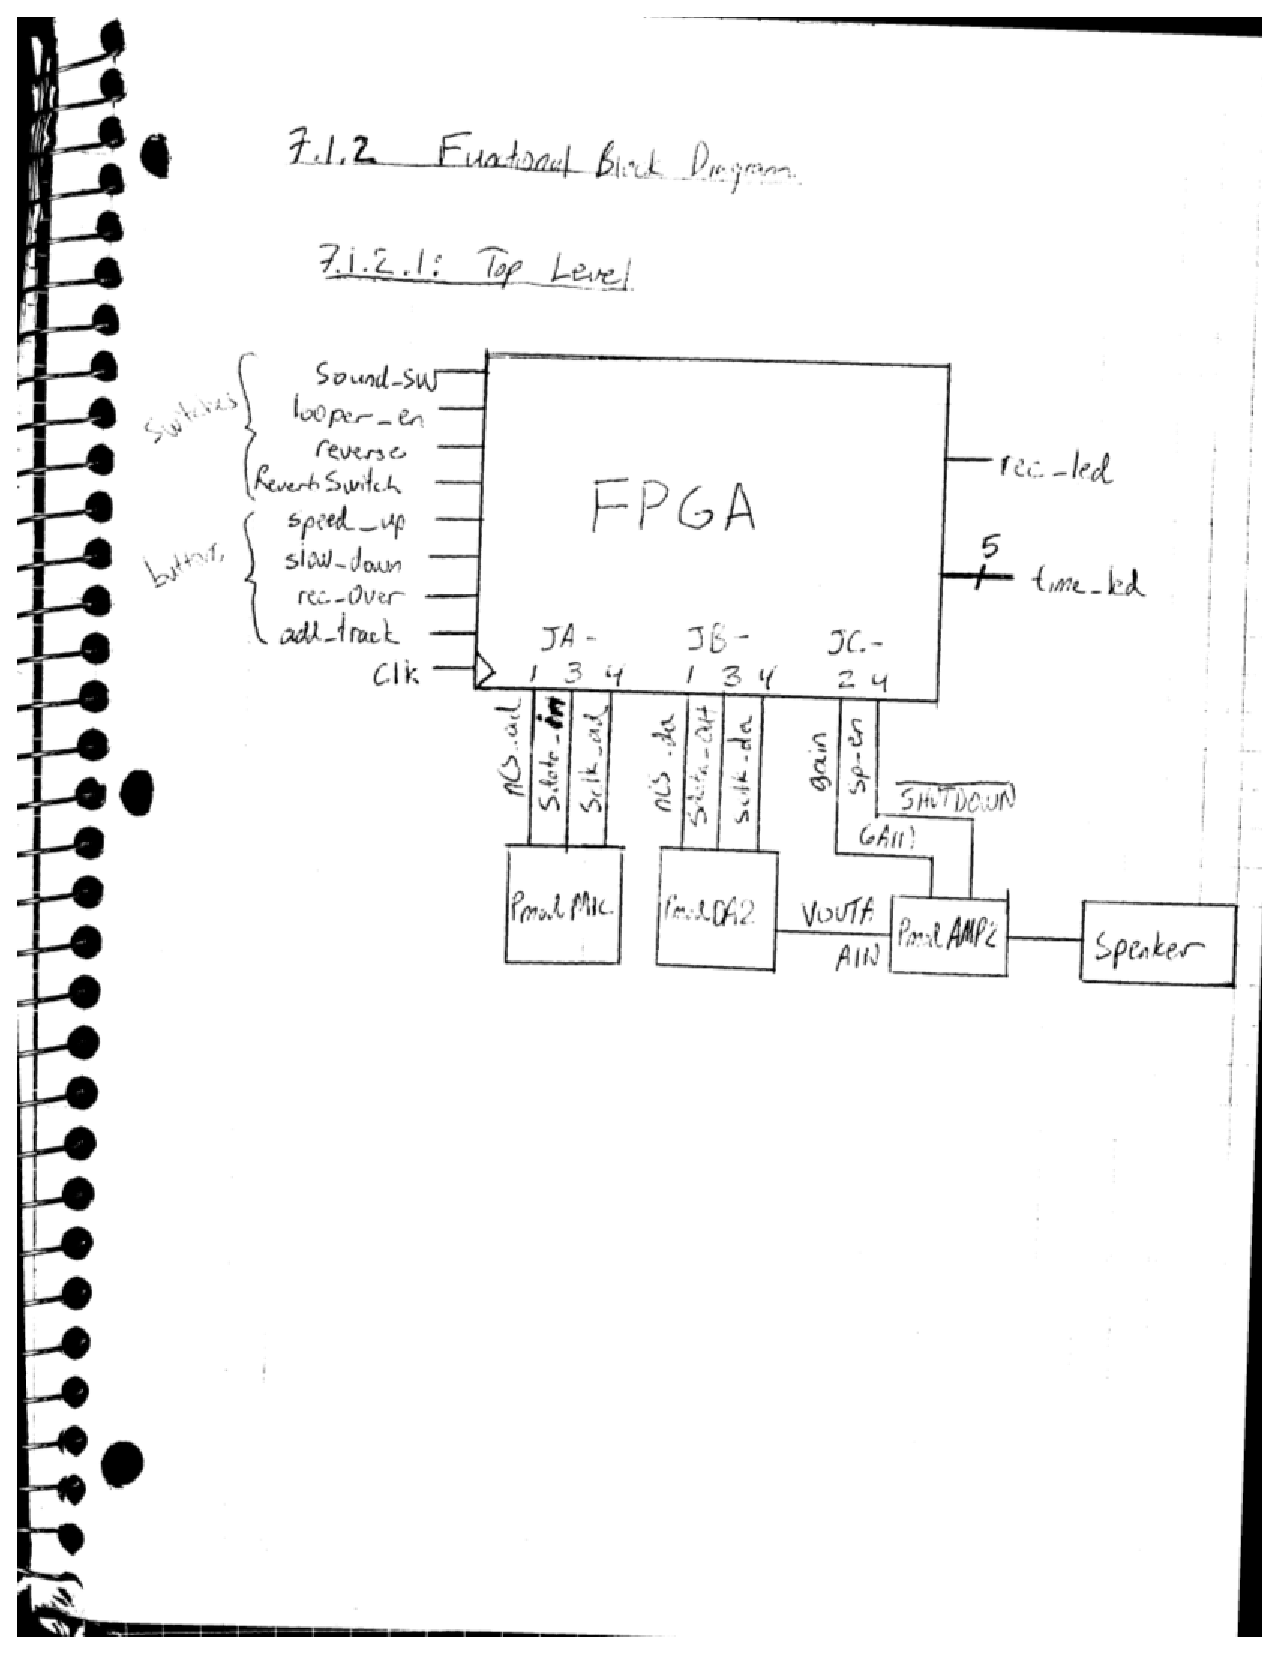
\includegraphics[width=0.75\textwidth, height=0.85\textheight]{toplevel_schem.eps}
\caption{Top Level Schematic}
\end{figure}

\begin{figure}[!htb]
\centering
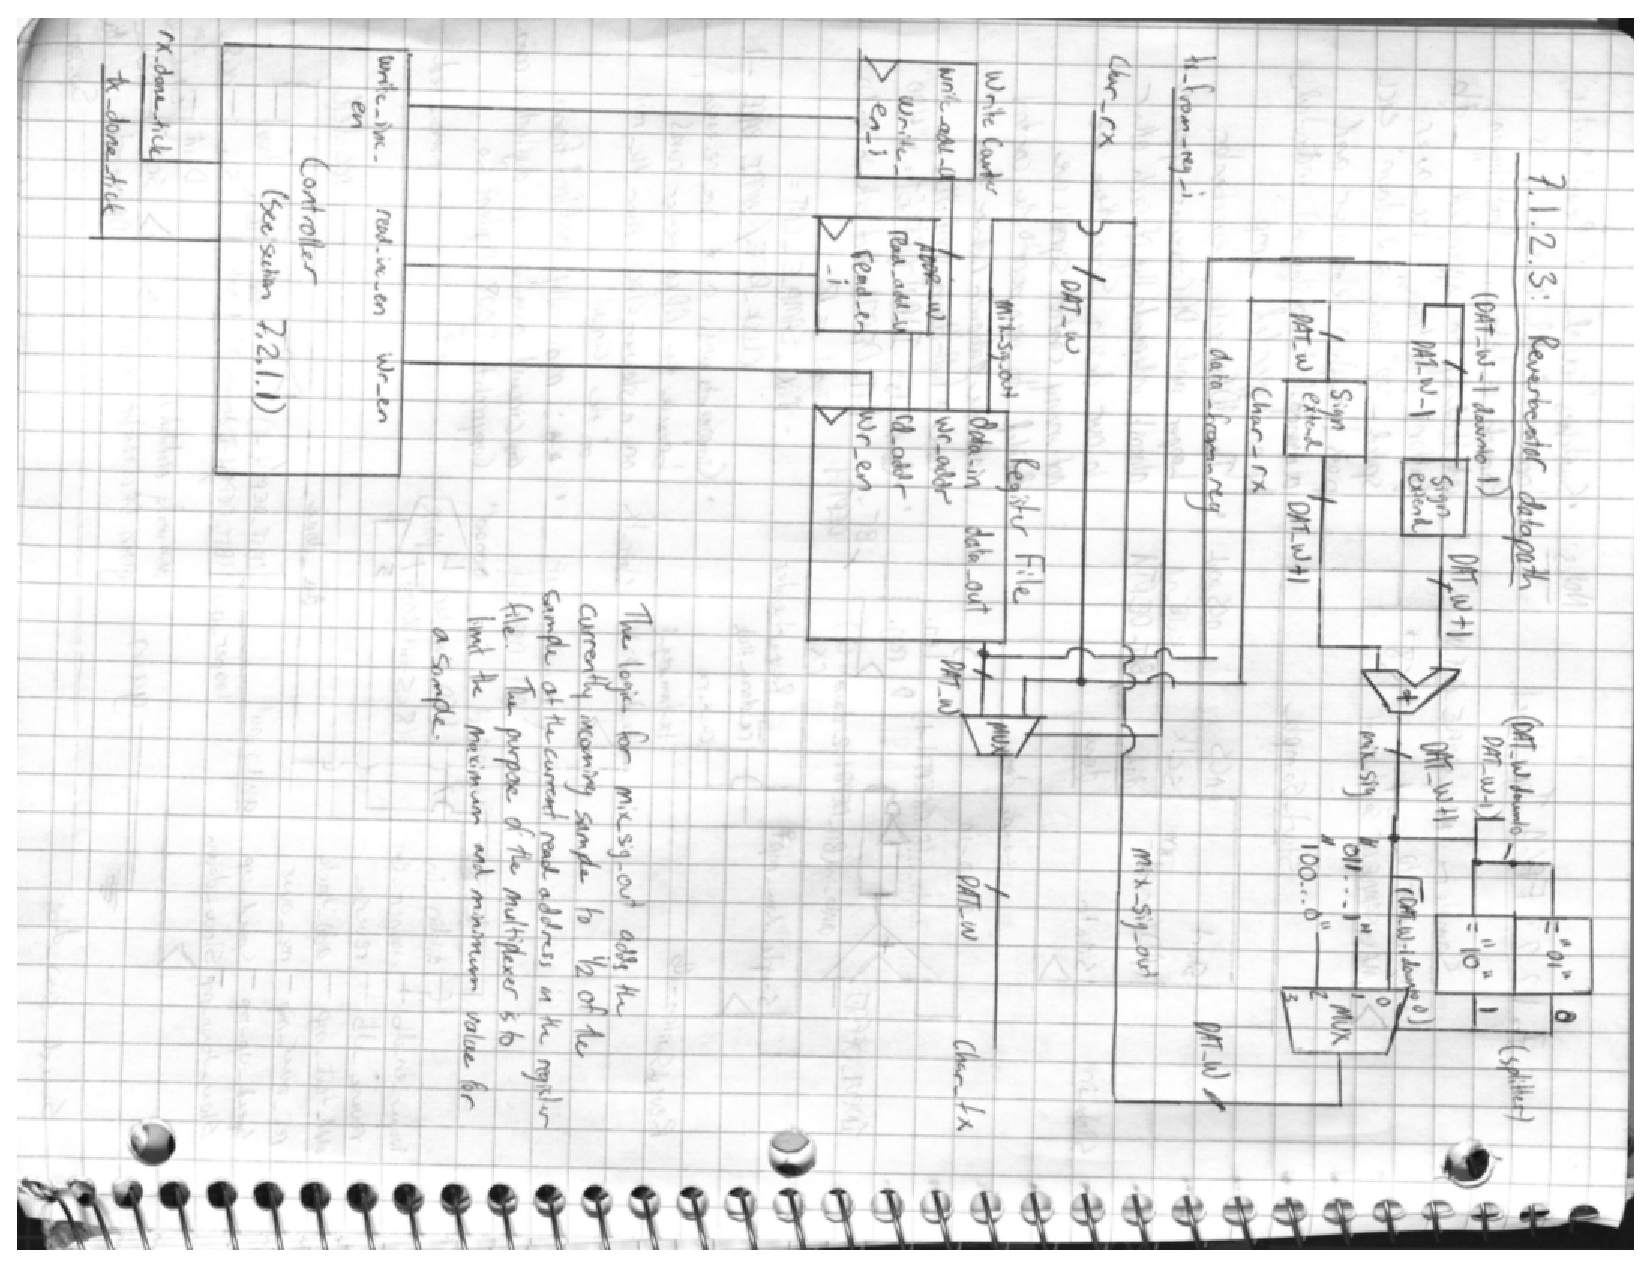
\includegraphics[width=0.5\textwidth, height=0.5\textheight, angle=90]{reverberator.eps}
\caption{Reverberator Top Level Diagram}
\end{figure}

\begin{figure}[!htb]
\centering
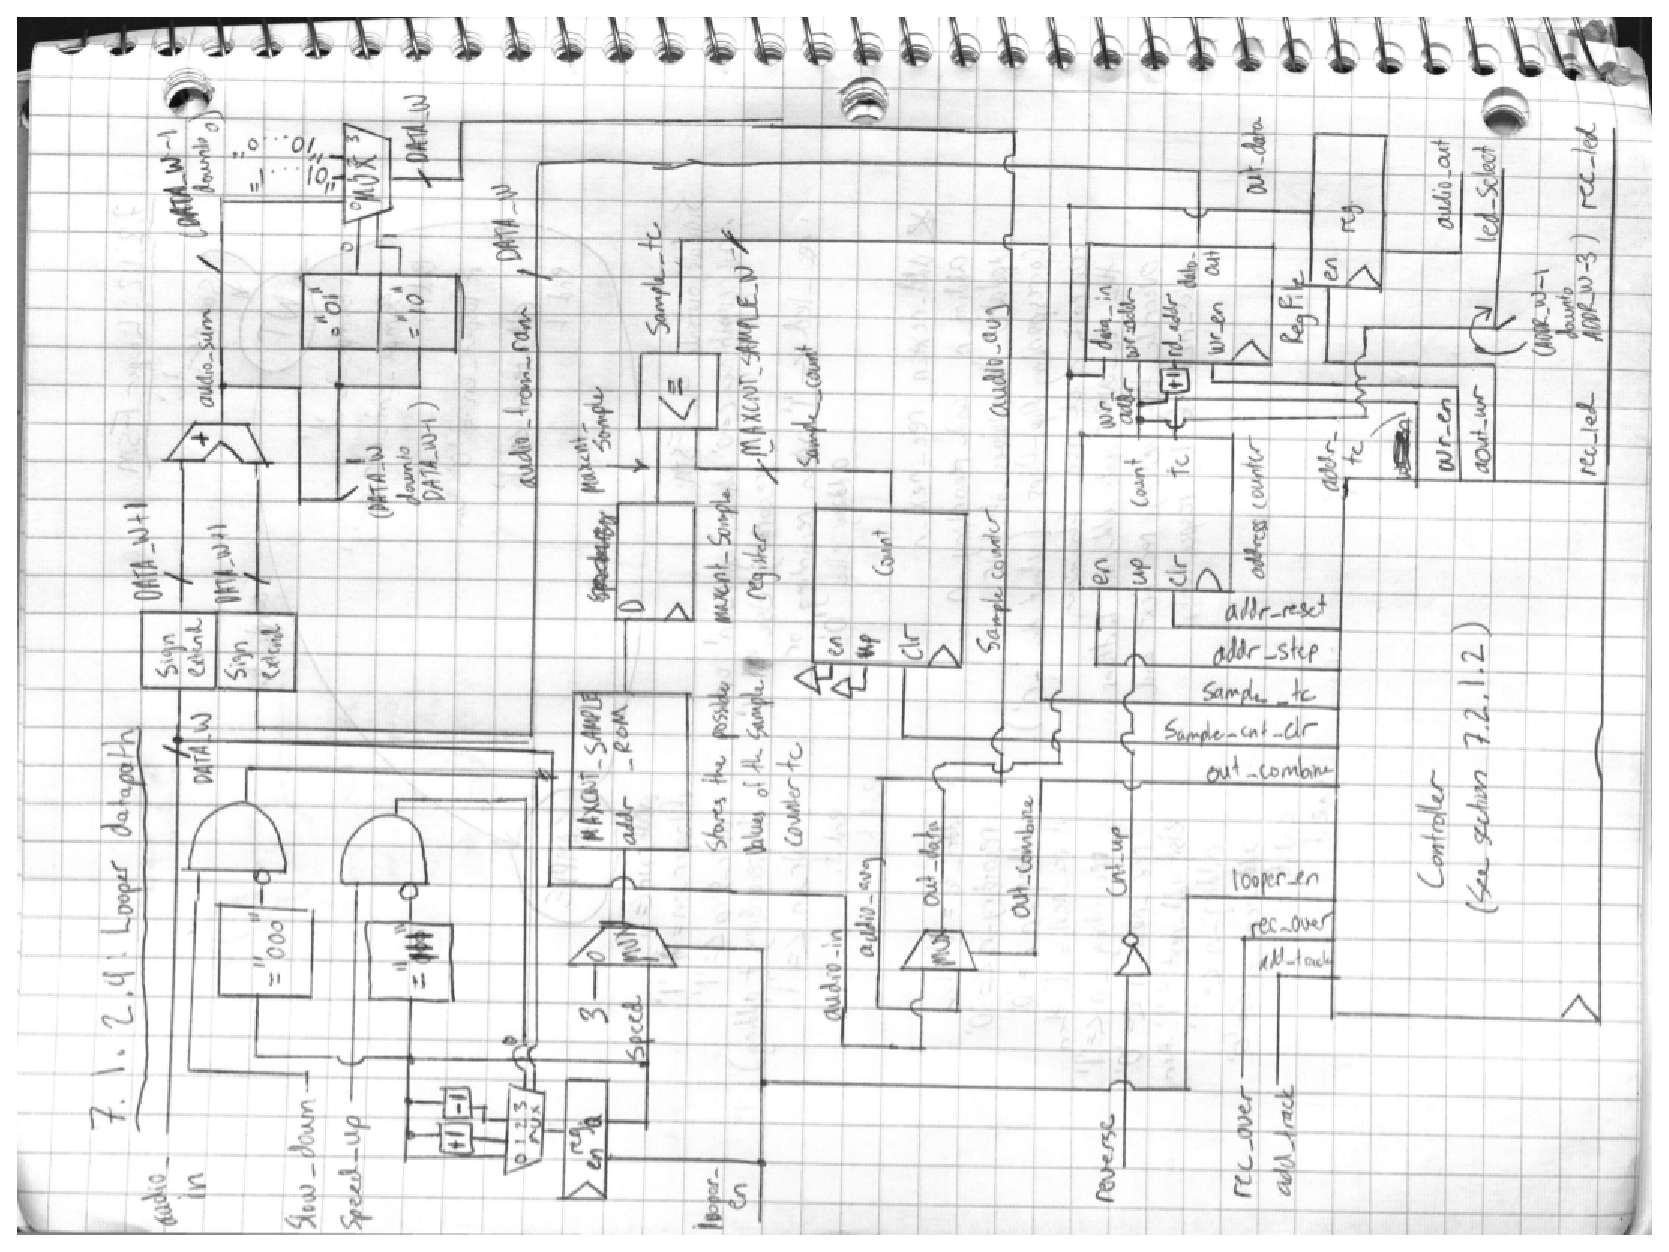
\includegraphics[width=.5\textwidth, height=.5\textheight, angle=270]{looper.eps}
\caption{Looper Top Level Diagram}
\end{figure}

\begin{figure}[h]
\centering
\includegraphics[width=0.5\textwidth, height=0.5\textheight, angle=270]{FPGAtop.eps}
\caption{FPGA Top Level Diagram}
\end{figure}

\begin{figure}[h]
\centering
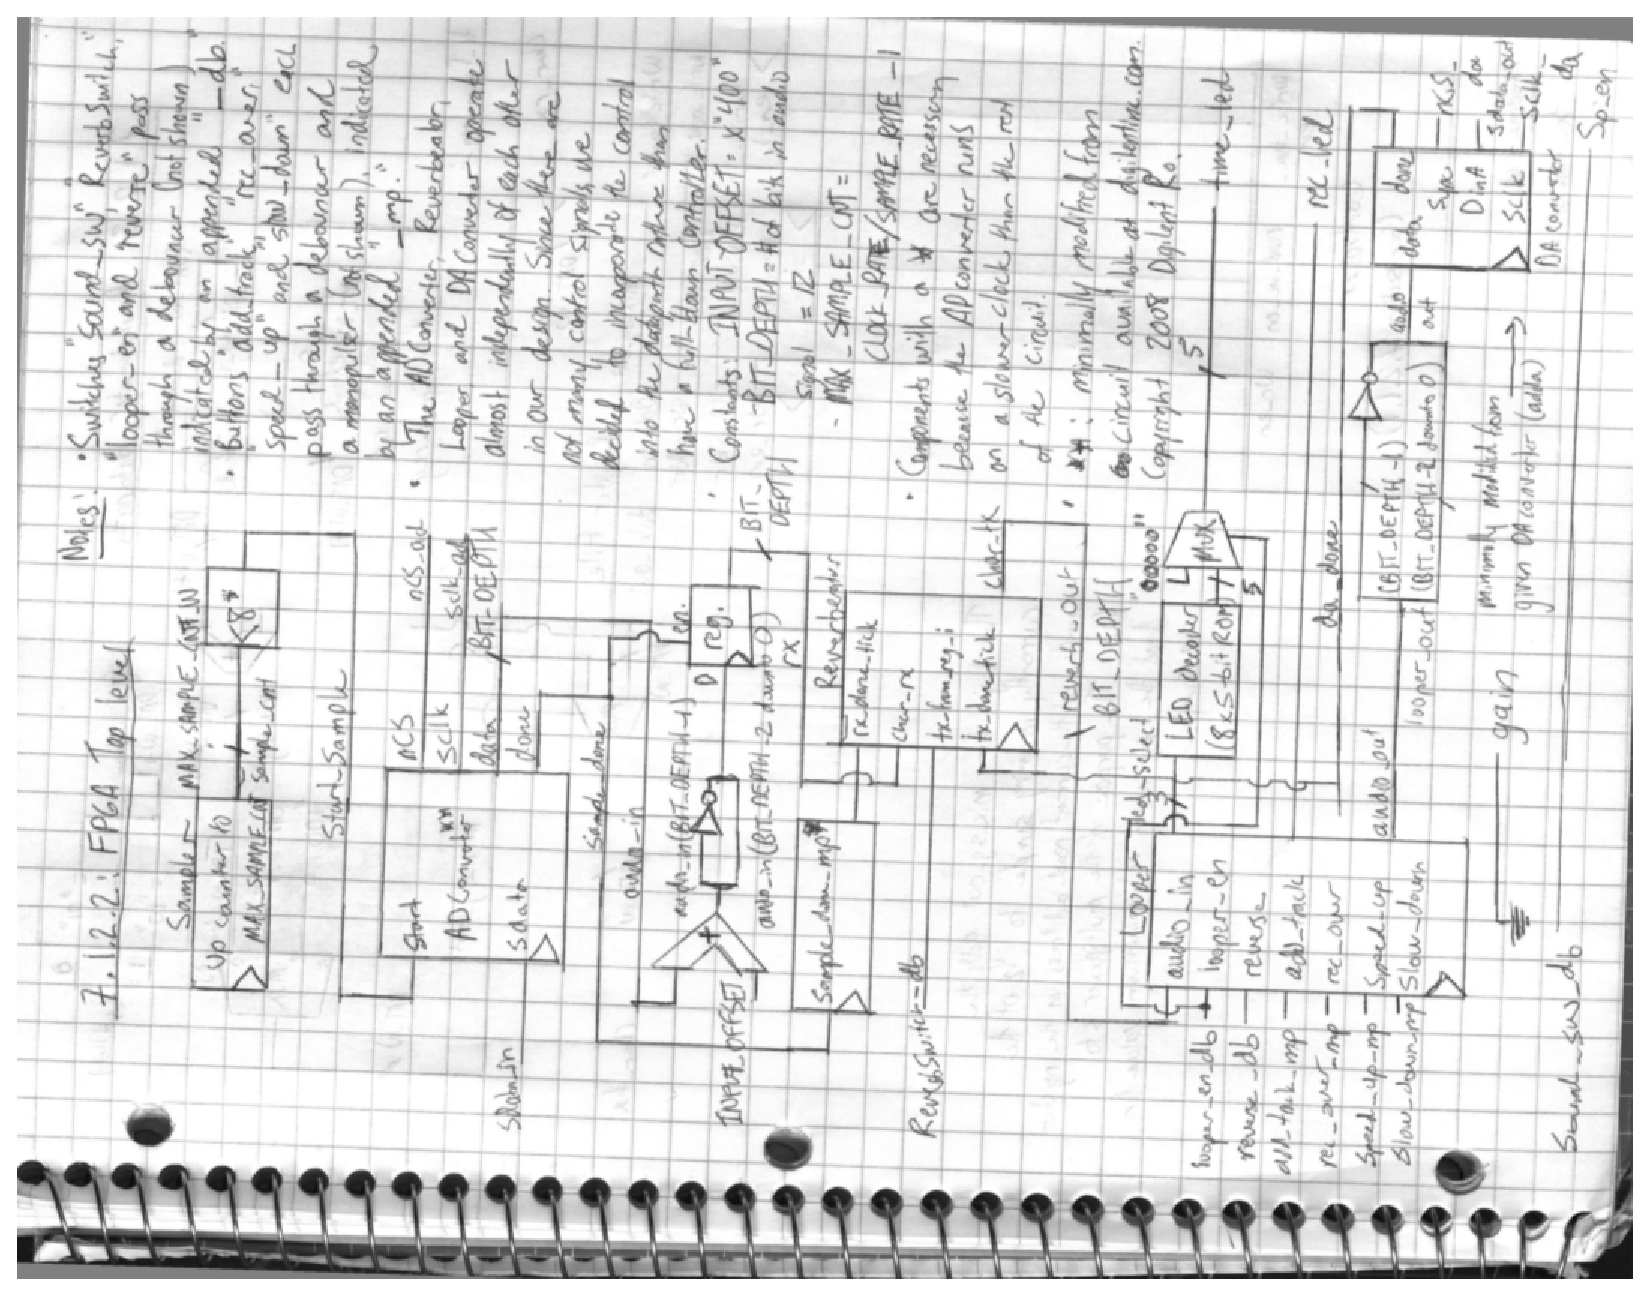
\includegraphics[width=0.5\textwidth, height=0.5\textheight, angle=270]{functional.eps}
\caption{Functional Top Level Diagram}
\end{figure}

\subsubsection{Parts List}
Xilinx PMOD AMP2
\\Xilinx PMOD DA2
\\Xilinx PMOD Mic
\\Xilinx Nexys 3 FPGA

\subsection{Programmed Logic}
\subsubsection{State Diagrams}

\begin{figure}[!htb]
\centering
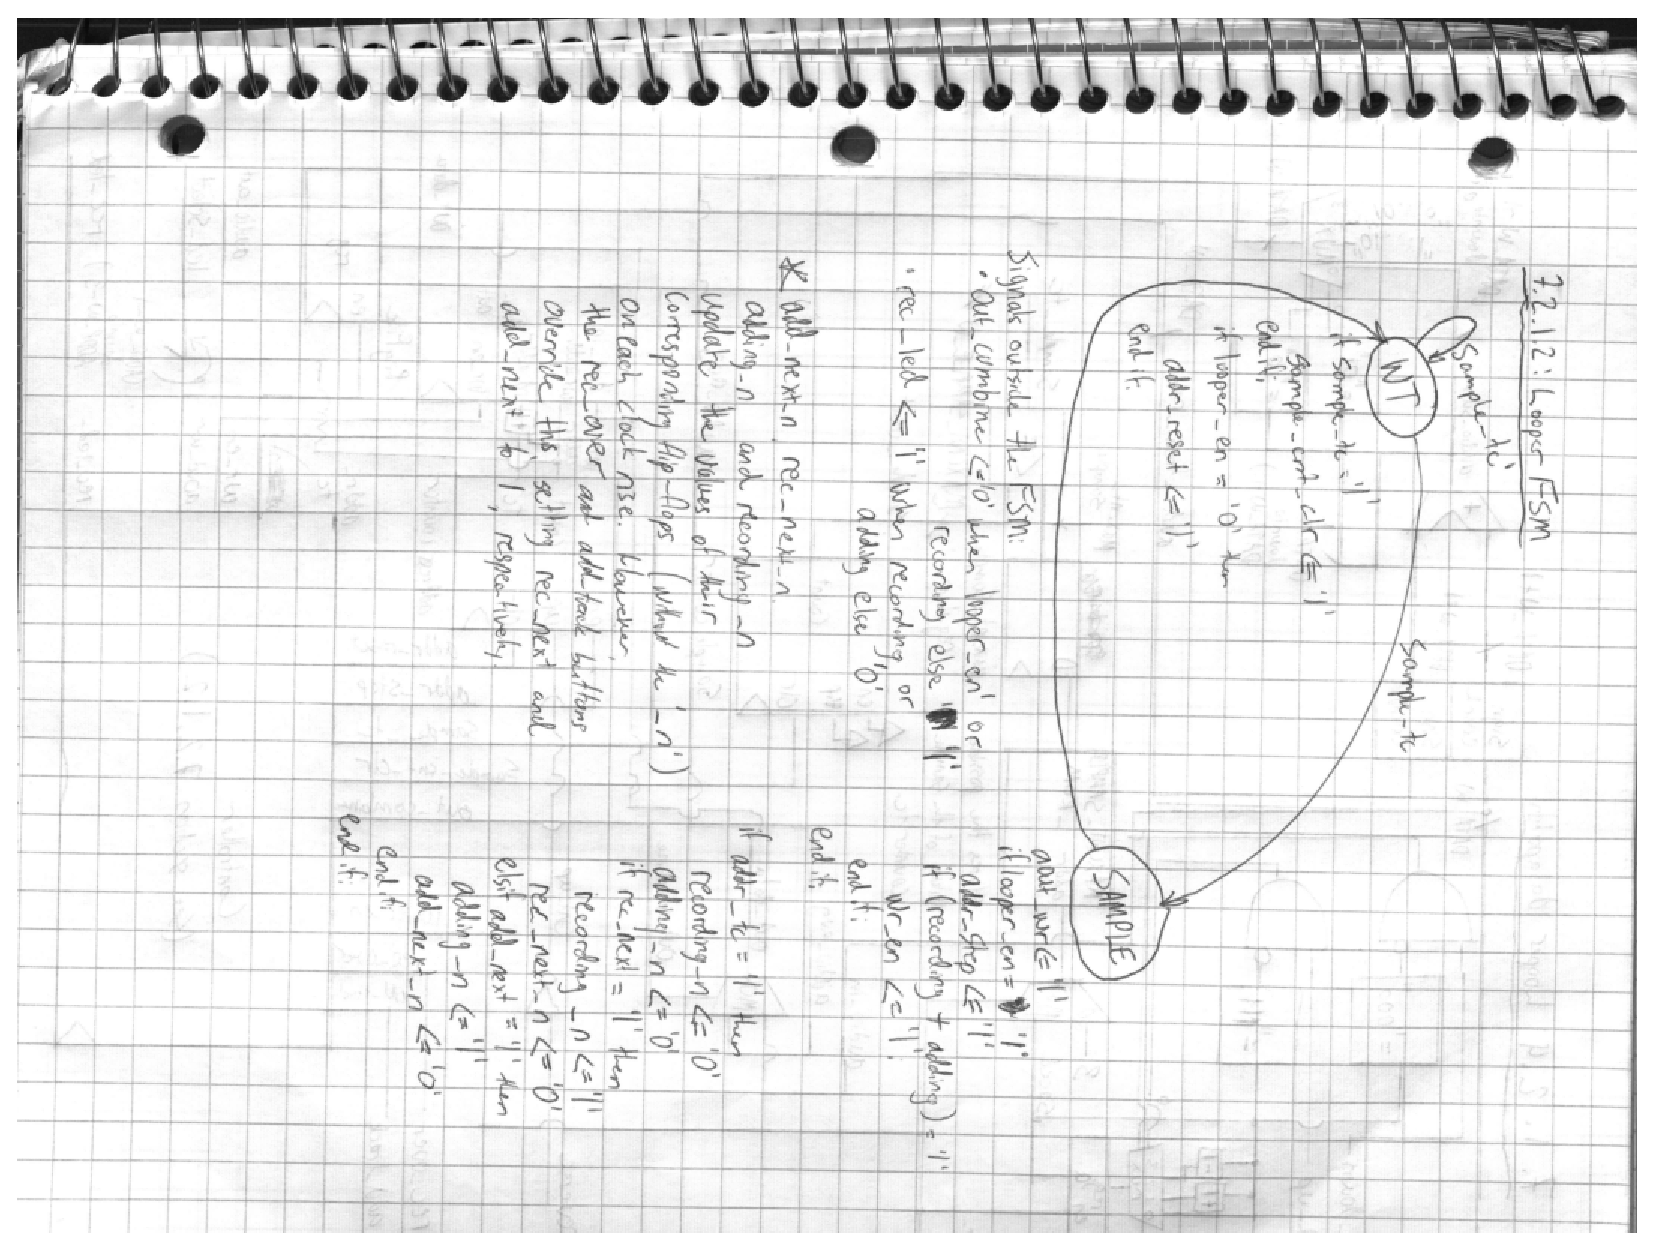
\includegraphics[width=1\textwidth, height=0.5\textheight, angle=90]{looperFSM.eps}
\caption{Looper Finite State Machine}
\end{figure}

\begin{figure}[!htb]
\centering
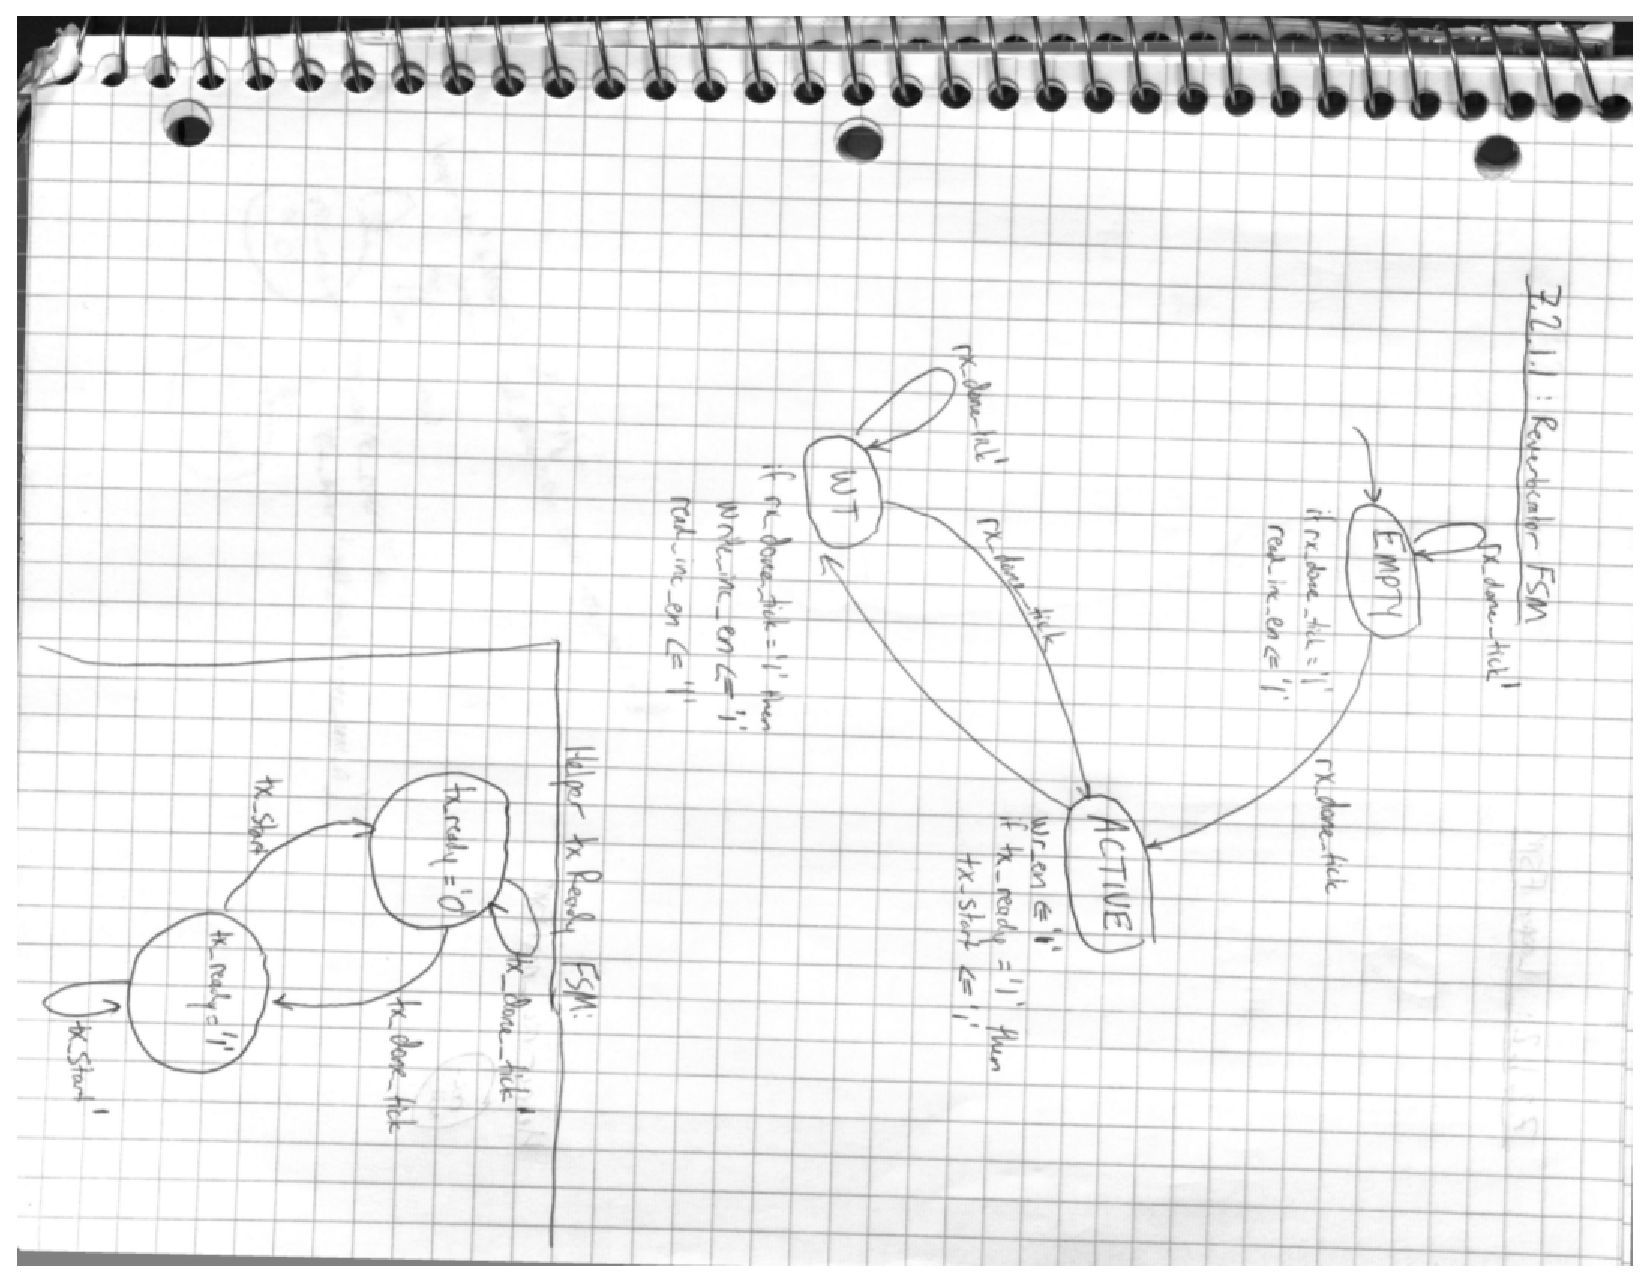
\includegraphics[width=1\textwidth, height=0.5\textheight, angle=90]{reverberatorFSM.eps}
\caption{Reverberator Finite State Machine}
\end{figure}



\subsubsection{VHDL Code}
\subsubsection{Resource Utilization}
\paragraph{}
Our design is heavy on memory and light on logic. We use 434 out of 9112 slice lookup tables, which is only 4\%. 

We use 485 LUT-flip-flop pairs, of which 178 have an unused flip-flop. Thus, we use 307 out of 18,224 flip-flops, which is only 1\%.

We use 23 out of 232 IO buffers, which is 9\%.
We use 30 out of 32 block RAM components. Since the block RAM was the limiting factor in our design, we set out to use as much of the available RAM as possible, and to distribute this storage between the reverberator and looper in an optimal way. We ended up having more block RAM to work with than we were expecting, so we also increased the sample rate in order to increase the sound quality.
\subsubsection{Critical Timing Path}
\paragraph{}
The critical timing path for the main clock has a delay of 6.260ns. This is the path that any entry of the reverberator's register file takes to reach the looper's register file (when both components are enabled). It passes through a multiplexer, a sign extender, an adder, a comparator and two more multiplexers before finally arriving at the looper's register file.
\subsubsection{Analysis of Residual Warnings}
\subsection{Waveform Graphs}
\begin{figure}[!htb]
\centering
\includegraphics[width=1\textwidth, height=0.5\textheight, angle=90]{reverb_sim.eps}
\caption{Waveform Graph}
\end{figure}
\end{document}
